\subsection*{Question 2.3}

In figure \ref{fig:q23a}, the original prediction trend,
$p(\mathbf{x}|\mathcal{C}_k)$ is displayed. In figure \ref{fig:q23b}
the prediction trend of Bayes classification is displayed. It can be
seen, that the two figures are very much alike, but some small
differences have happened.

\begin{figure}[!htbp]
  \centering
  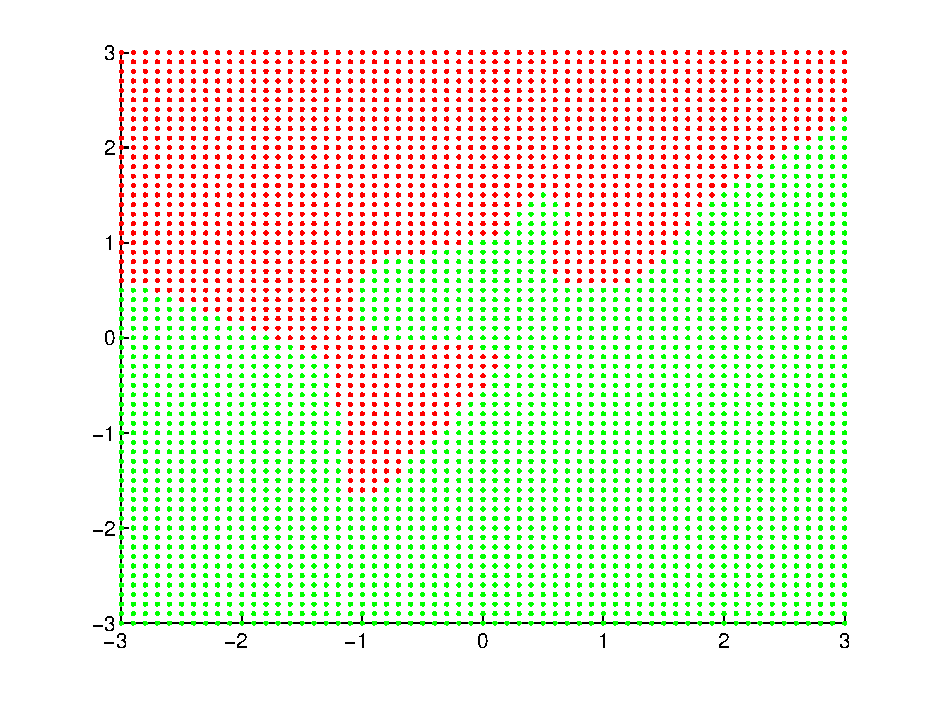
\includegraphics[width=0.6\textwidth]{./images/q23a.pdf}
  \caption{The original prediction trend, $p(\mathbf{x}|\mathcal{C}_k)$}
  \label{fig:q23a}
\end{figure}

\begin{figure}[!htbp]
  \centering
  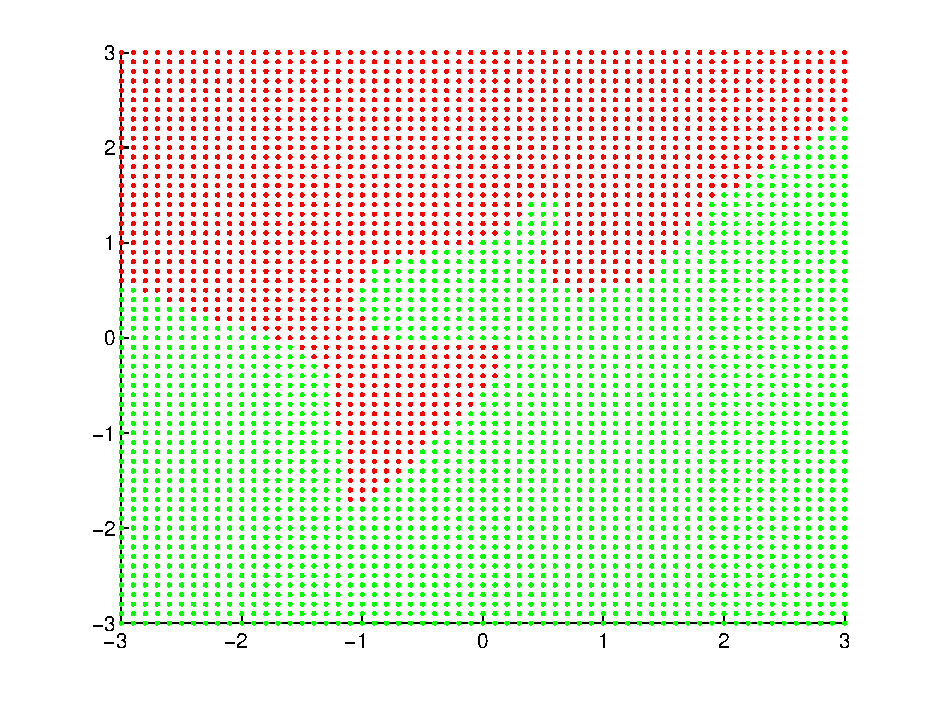
\includegraphics[width=0.6\textwidth]{./images/q23b.pdf}
  \caption{The prediction trend of the Bayes classifikation, $p(\mathbf{x}|\mathcal{C}_k)$}
  \label{fig:q23b}
\end{figure}

As it can be seen, in figure \ref{fig:q23c}, chancing the prior of one of
the classes. Makes it more or less dominent.

\begin{figure}[!htbp]
  \centering
  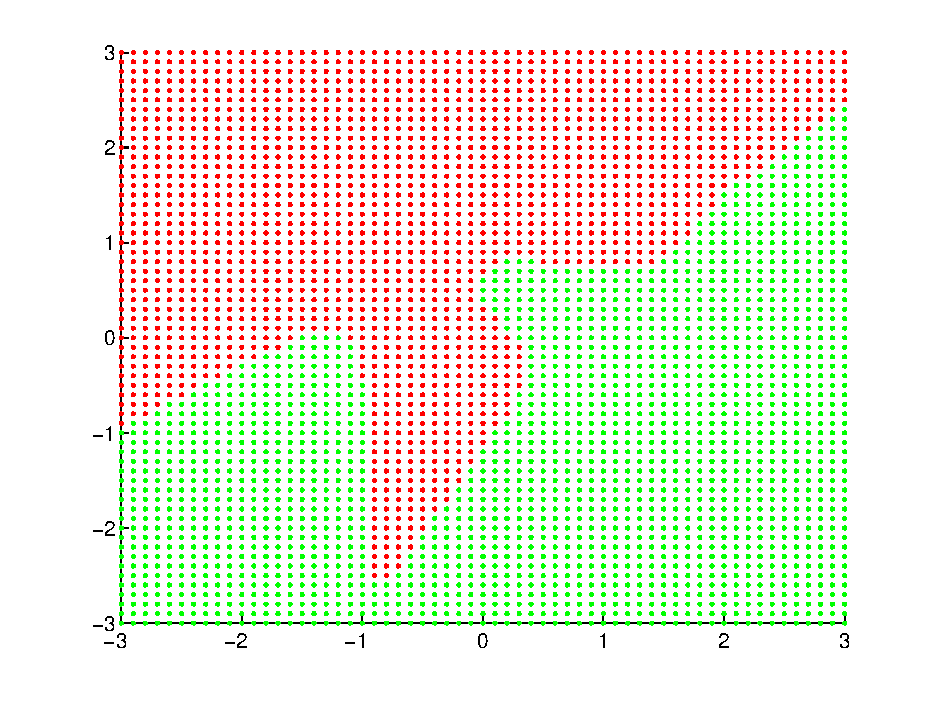
\includegraphics[width=0.6\textwidth]{./images/q23c.pdf}
  \caption{The prediction trend of the Bayes classification, where class one, have a prior of 1.5}
  \label{fig:q23c}
\end{figure}
